\section{Système biologique}
\label{sec:sys_bio}

Les systèmes biologiques sont au centre de l'activité des organismes. La définition de système biologique est très vaste et lié au domaine et au contexte scientifique. Ainsi, dans cette partie, je définirai les systèmes biologiques dans le domaine de la génomique comparée des procaryotes et le replacerai dans le contexte des travaux de recherche que j'ai réalisés. Je reviendrai aussi sur l'état de l'art des méthodes bioinformatique de détection de tels systèmes, puis je décrirai plus précisément un type particulier système, qui a été mon sujet d'application pour mes développements méthodologique, les systèmes de défense contre les phages.

\subsection{Définition et intérêt}

Un système biologique correspond à un ensemble d'éléments biologiques qui interagissent ensemble pour réaliser un ensemble de fonctions, aboutissant à opérer un processus. Dans le contexte de la génomique comparée des procaryotes, ces éléments sont les portions d'ADN qui vont coder  les protéines ou en réguler l'activité.
Ainsi, nos systèmes biologiques correspondent à un ensemble de gènes et de régulateurs impliqués dans un processus cellulaire, on peut alors trouver le terme de système génétique. Les systèmes vont être plutôt catégorisés en fonction du type de processus auxquels ils participent. Par exemple, les systèmes qui participent à la conjugaison sont des systèmes conjugatifs.

La description et l'étude de ces systèmes est essentielle, car une fois identifiés, ils permettent de caractériser une voie métabolique ou un complexe macromoléculaire dans l'organisme \cite{alberts_cell_1998}. De plus, les systèmes sont régulièrement associés à des îlots génomiques (cf. \autoref{sec:ilot}), comme les systèmes de sécrétion de type III et VI associés aux îlots de pathogénicités\cite{pallen_bacterial_2007}. L'identification de tels systèmes dans les GIs est essentielle à la compréhension de l'adaptation et de la diversité des écosystèmes procaryotes. Néanmoins, leur identification n'est pas systématique, car décrire ces systèmes n'est pas trivial.

Premièrement, ces systèmes comportent des composants dont l'importance varie : certains sont indispensables, tandis que d'autres sont facultatifs ou spécifiques à certaines niches écologiques. Par exemple, la réparation de l’ADN repose sur RecA, une protéine clé de la recombinaison homologue, mais peut aussi emprunter des voies alternatives, comme le système RecBCD chez \textit{Escherichia coli} ou AddAB chez \textit{Helicobacter pylori}\footnote{Bactérie pathogène connue pour son rôle dans les infections gastriques et notamment dans les ulcères de l'estomac.} \cite{dillingham_recbcd_2008}. Ensuite, de nombreux composants partagent des homologues avec d’autres systèmes, et même de systèmes très différents, rendant leur classification complexe. C’est notamment le cas du système de sécrétion de type VI, qui présente des similitudes structurelles avec les phages à queue contractile, suggérant une origine évolutive commune \cite{coulthurst_type_2013}. La dynamique évolutive des systèmes est également hétérogène. Certains composants sont fortement conservés, tandis que d'autres évoluent rapidement sous l'effet de pression de sélection. C'est le cas des systèmes de défense (cf. \autoref{sec:def}), tels que les systèmes CRISPR-Cas, dont la diversité des protéines Cas (permettent de découper l'ADN viral) reflète une adaptation continue aux menaces \cite{makarova_comparative_2013}. Cette variabilité complique alors l’identification des homologues par la seule comparaison de séquences.

Pour surmonter ces difficultés, l'identification de systèmes repose sur la combinaison de la recherche des composants et sur l'organisation en contexte. En effet, comme nous l'avons vu dans les \autoref{sec:structure_org} et \autoref{sec:fn_reg}, les gènes codant des protéines impliqués dans un même processus (ou systèmes ici) ont tendance à rester colocaliser, notamment dans les opérons. En s'appuyant sur ces propriétés, on peut alors identifier des systèmes connus et même inconnus (mais proches) chez les organismes.

\subsection{Méthode de détection}

Avant les années 2000, la recherche de systèmes biologiques était basée sur des approches phylogénétiques, en recherchant des homologues, ou par de l'annotation manuelle de régions d'intérêt comme les GIs. Des outils se sont ensuite développés pour détecter différents systèmes : les systèmes conjugatifs, les systèmes de sécrétion, les systèmes de défenses contre les phages (\autoref{sec:def}) et les systèmes métaboliques. Leur évolution a suivi une trajectoire marquée par des avancées méthodologiques, passant de simples bases de données statiques à des modèles probabilistes et des approches d’intelligence artificielle.

Les premiers outils pour la recherche de systèmes spécifiques, annotent les génomes pour "allumer" les gènes codant pour une fonction d'intérêt connue à partir d'une base de données de référence. En 2008, l'outil et la base de données liée ICEberg \cite{bi_iceberg_2012} permet d'identifier les ICEs (cf. \autoref{sec:evo_hz}) à partir d'une base de données de protéines, annotées manuellement, et d'un alignement avec BLASTp sur les génomes. Bien que la base de données soit régulièrement mise à jour \cite{wang_iceberg_2024}, il reste qu'ICEberg n'est pas adapté à la détection des ICEs divergents, et donc limite son utilisation à la détection de système bien caractérisés. SecReT4 \cite{bi_secret4_2013} a proposé une base de données spécifique pour la détection des systèmes de type IV (T4SS). Bien qu’utile, cette approche était limitée par la nécessité de mises à jour régulières et une couverture incomplète des systèmes de sécrétion existants.

En 2011, antiSMASH \cite{medema_antismash_2011} a marqué un tournant en permettant une annotation automatique des clusters de gènes biosynthétiques (BGCs pour \textit{Biosyntetic gene cluster} en anglais). Son succès s’explique par sa large base de données de profils HMM permettant une annotation plus vaste et de meilleure qualité des gènes. De plus, il détecte un large éventail de BGCs, notamment les NRPS (peptides non ribosomiques), les PKS (polykétides) et d’autres métabolites secondaires. Concernant les systèmes de sécrétion, T4SEpre \cite{wang_prediction_2014} propose également d'utiliser des modèles, cette fois des profils pour détecter les systèmes T4SS. Malgré ces améliorations, ces outils ne prennent pas en compte l'organisation génomique.

En 2014, MacSyFinder  est publié \cite{abby_macsyfinder_2014} et va aussi marquer une nouvelle étape dans la recherche de systèmes. MacSyFinder va  proposer d'utiliser une base de données, ici HMM, pour annoter les gènes dans les génomes. Par contre, il va apporter la notion de modèle de système pour décrire les composants du système et son organisation génomique. L'intérêt du modèle est de pouvoir décrire de façon fine les systèmes. Un modèle est censé être une représentation exhaustive et spécifique d'un type de système. C'est pourquoi, par exemple, il est possible de décrire certains gènes comme interdit, afin de discriminer les systèmes homologues (\autoref{fig:macsyfinder}). De plus, la composition du modèle n'est pas stricte, ce qui permet de retrouver des systèmes homologues avec diverse composition. Dans les modèles, on retrouve aussi l'information de colocalisation, où 2 gènes doivent être dans un espace génique spécifique et limité\footnote{MacSyFinder introduit différent mot clé pour ajuster les modèles, dont \textit{loner} et \textit{multi\textunderscore loci} qui permettent de passer outre la colocalisation.}. MacSyFinder se veut également flexible et est utilisable pour détecter tous types de systèmes. Ainsi, en utilisant les modèles TXSScan \cite{abby_identification_2016} on détecte les systèmes de sécrétion, TFFScan \cite{denise_diversification_2019} pour les filaments de type IV, CONJScan \cite{cury_integrative_2017} pour les systèmes de conjugaison. Bien que MacSyFinder et ses modèles permettent une identification plus fine, il reste qu'ils sont basés sur les systèmes connus et qu'ils ne permettent pas de détecter des systèmes inconnus. Toutefois, certains modèles sont plus flexibles et correspondent à un ensemble de type de système d'une même catégorie. Ces modèles peuvent permettre de retrouver des systèmes inconnus, mais ils doivent ensuite être prouvés. 

\begin{figure}[htbp]
    \centering
    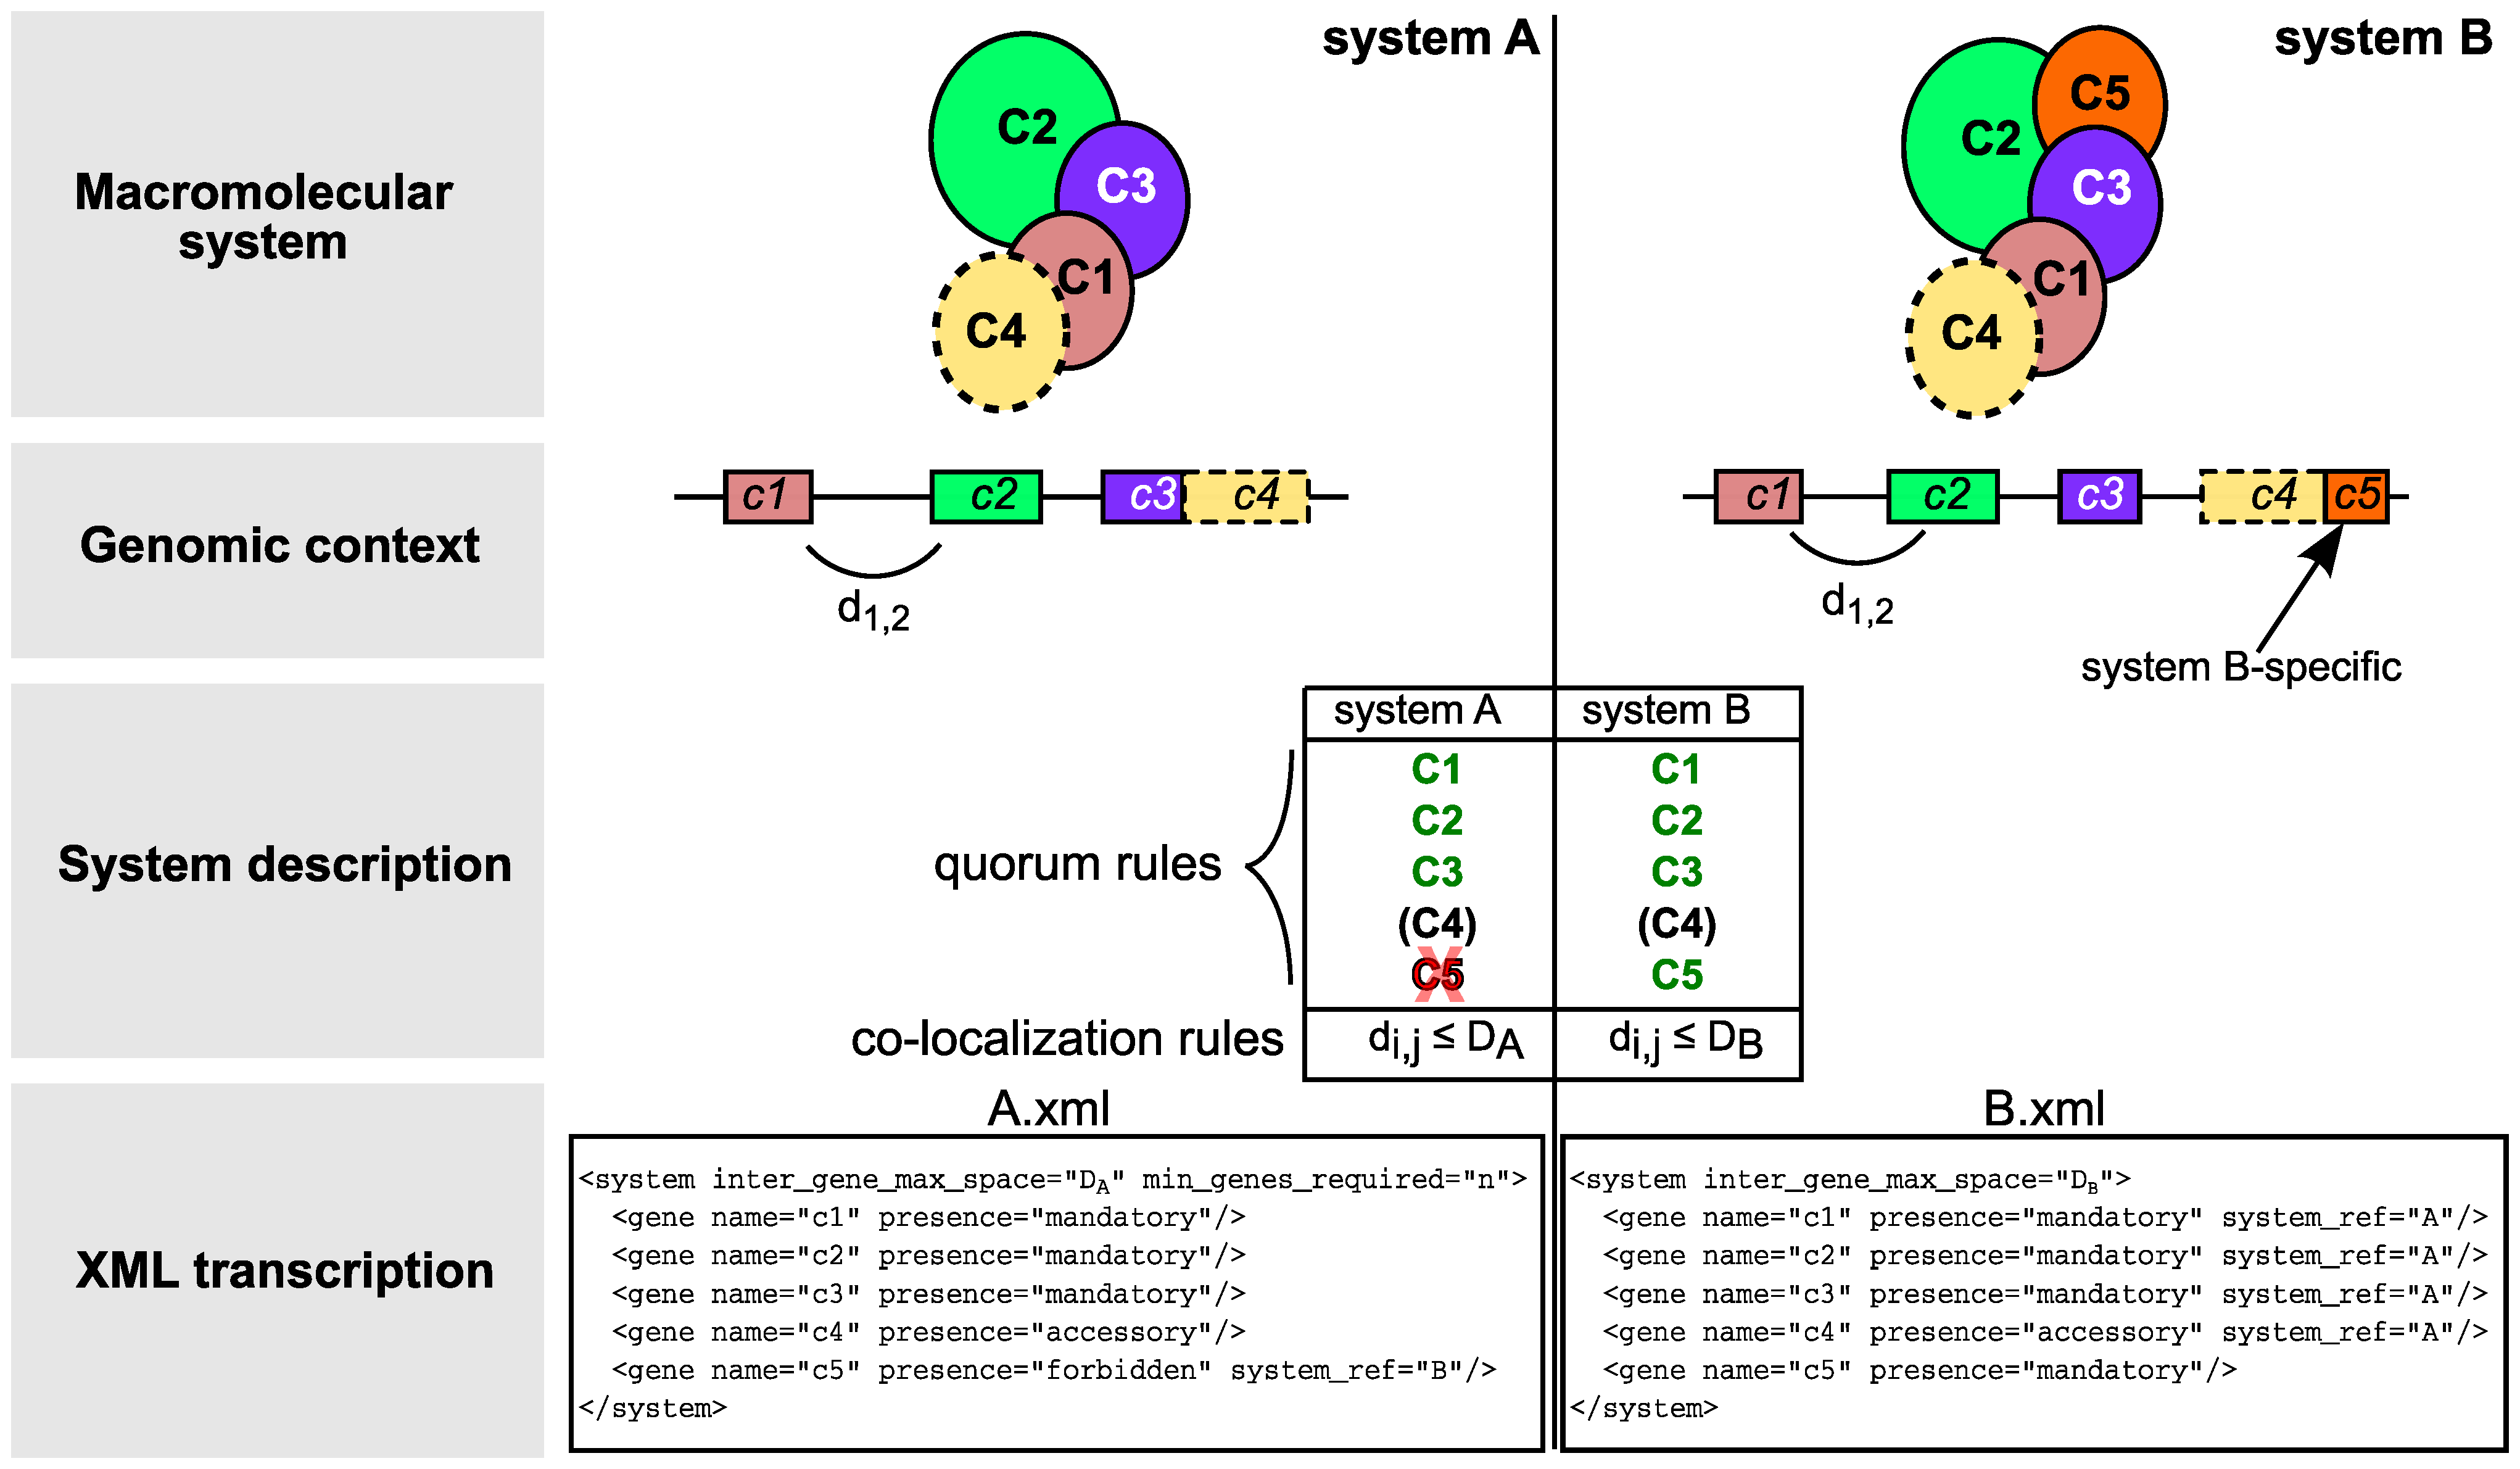
\includegraphics[width=0.75\linewidth]{images/macsyfinder.png}
    \caption{Expemple de modélisation de systèmes dans MacSyFinder. Extrait de \cite{abby_macsyfinder_2014}}
    \label{fig:macsyfinder}
\end{figure}

Des méthodes récentes tirent parti du développement du machine learning et de l'intelligence artificielle. DeepBGC \cite{hannigan_deep_2019} utilise des modèles de \textit{deep learning} et des approches de traitement du langage naturel pour prédire les  BGCs,  Cependant, DeepBGC nécessite une puissance de calcul importante et n’était pas aussi facilement accessible que des outils plus classiques. En 2021, GECCO \cite{carroll_accurate_2021} a amélioré la classification des BGCs en utilisant des réseaux de gènes (modèle \textit{deep learning}), ce qui a permis d’affiner encore davantage la précision des prédictions, bien que son utilisation soit plus complexe que celle d’antiSMASH. Du côté des systèmes de sécrétion, l'outil T4SEpp \cite{hu_t4sepp_2024} utilise des méthodes d'apprentissage automatique, améliorant la sensibilité et la spécificité de la prédiction. Ces méthodes, basées sur le \textit{machine learning}, ont l'intérêt de permettre la découverte de systèmes encore non décrits. Toutefois, il reste que ces méthodes demandent une phase d'apprentissage, ce qui augmente les ressources nécessaires et peut rendre l'outil moins accessible à la communauté non initiée aux méthodes d'apprentissage. 

\subsection{Systèmes de défense aux phages}
\label{sec:def}

Ces dernières années, l'intérêt pour les systèmes de défense aux phages a été croissant (6 publications en 2007 contre 241 en 2024). Des outils et bases de données ont été  développés pour les rechercher  dans les génomes et les analyser. Dans cette partie, nous reviendrons sur l'aspect biologique de ces systèmes en décrivant les systèmes les plus connus, puis nous reviendrons sur les méthodes disponibles pour leur identification.

\subsubsection{Phages : retour sur les virus de bactéries}
\label{sec:phage}
Les virus de bactérie, appelés bactériophages ou phages, ont été observés pour la première fois en 1915 et officiellement décrits par Félix D'Herelle. Les phages mesurent entre 20 et 200 nm prennent des formes et des compositions (ADN ou ARN, simple brin ou double brin) très diverses (\autoref{fig:phages}). Chaque phage est associé à un spectre d'hôte spécifique, \textit{i.e.}, il ne peut  contaminer  un nombre limité et défini d'espèces procaryotes dans le spectre. 

\begin{figure}[htbp]
    \centering
    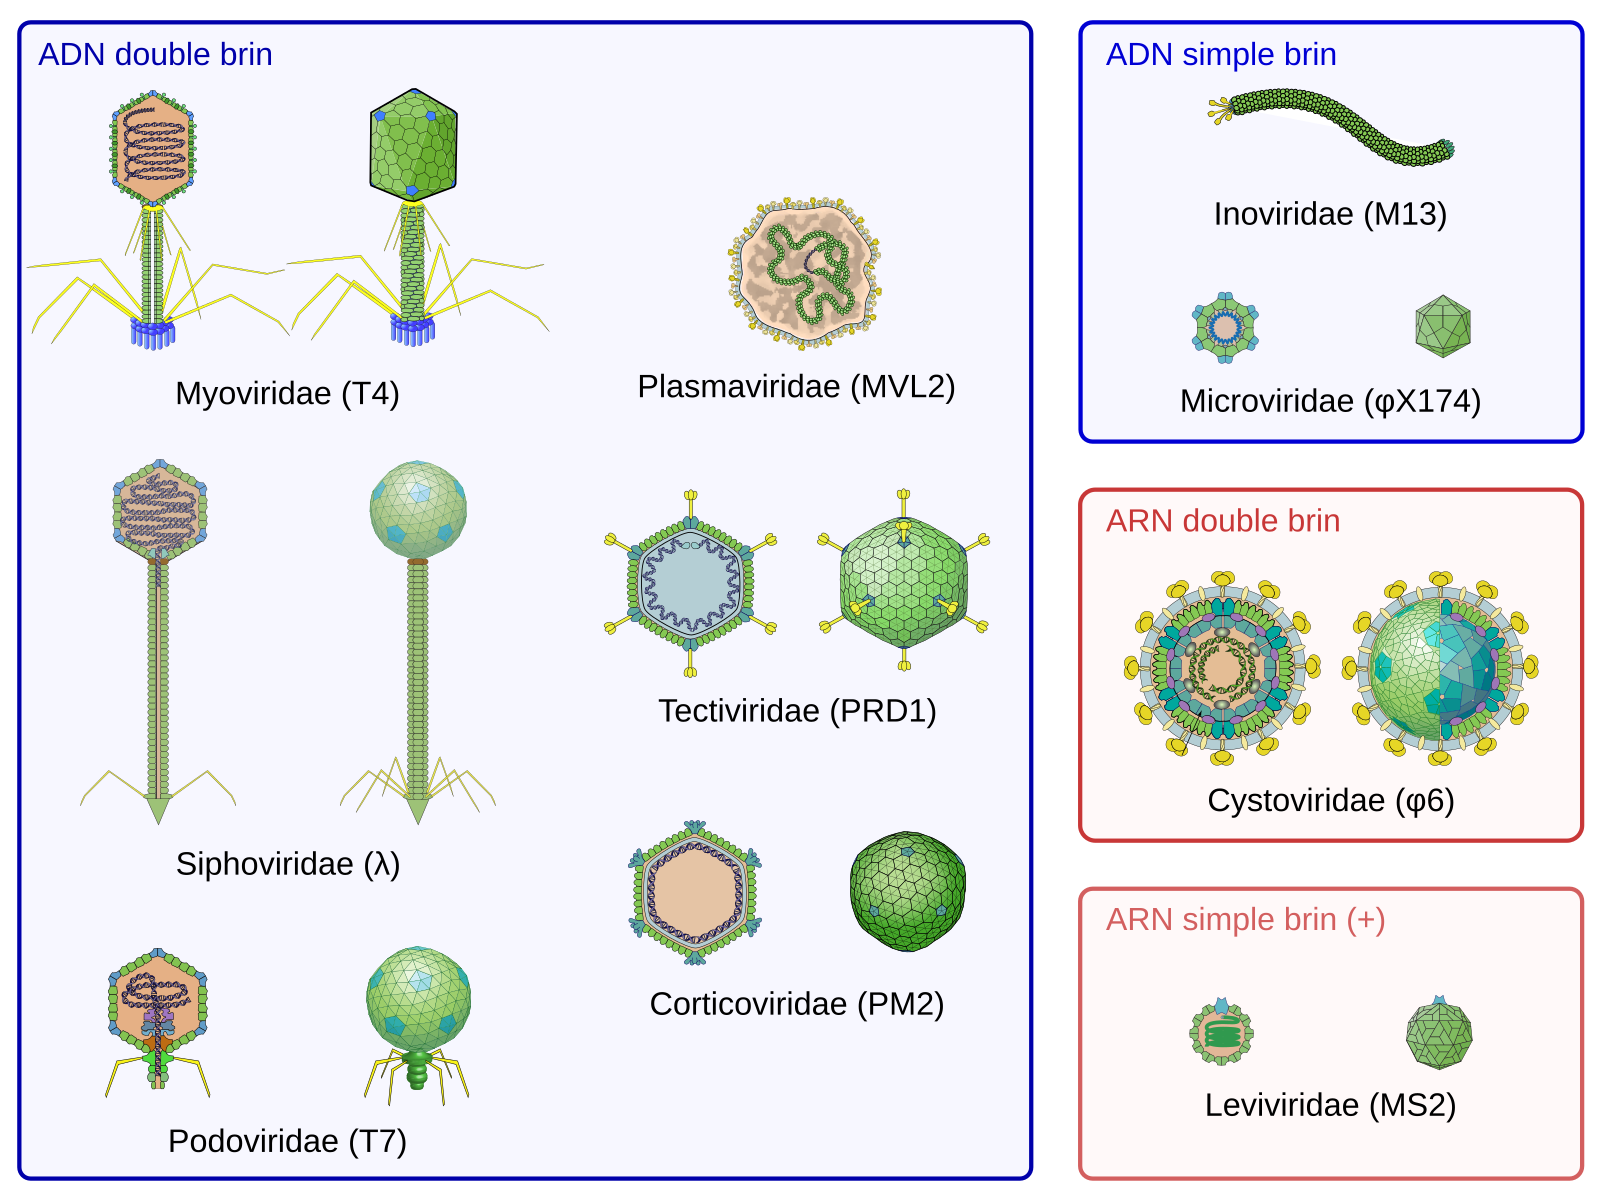
\includegraphics[width=0.75\linewidth]{images/phages.png}
    \caption[Diversité morphologique parmi les phages]{Philippe Le Mercier - ViralZone SIB Swiss Institute of Bioinformatics}
    \label{fig:phages}
\end{figure}

Les phages ne sont pas capables de répliquer leur propre matériel génétique, c'est pourquoi ils infectent les cellules procaryotes, afin d'utiliser les systèmes de réplication de l'hôte. Une fois que le matériel a été répliqué (des milliers de fois), les nouveaux phages seront libérés dans l'environnement en lysant la cellule (ouverture de la paroi). Le cycle d'infection, réplication, libération existe sous 2 formes définissant 2 catégories de phages \autoref{fig:transduction}. Le cycle lytique, pratiqué par les phages virulents, correspond à un cycle court où le phage détruit l'hôte à la fin de sa réplication. Le cycle lysogénique, pratiqué par les phages tempérés, réfère à un phage qui va rester dans la cellule pendant plusieurs cycles de réplication de l'hôte. Dans ce cas, le matériel génétique peut s'intégrer au chromosome de l'hôte et se répliquer avec lui, on parle de région prophagique, ou rester dans le cytoplasme sous forme d'épisome et se répliquer indépendamment comme un plasmide.

Quel que soit le cycle, l'infection de l'organisme par un phage signe sa destruction future. Les procaryotes ont donc développé un arsenal pour se protéger : les systèmes de défense contre les phages \cite{makarova_comparative_2013}. Aujourd'hui les phages sont utilisés comme une thérapie alternative aux antibiotiques, il est donc essentiel de connaitre la résistance possible des bactéries pathogènes aux phages avant de les utiliser \cite{cui_current_2024}.

\subsubsection{Système de défense contre les phages}

Un système de défense contre les phages (que nous raccourcirons en systèmes de défense dans cette partie) correspond à un ensemble de protéines qui vont empêcher l'action du phage et donc empêcher la destruction de la cellule. Dans la nature, il en existe une grande diversité et un organisme n'est capable d'en utiliser seulement une partie. 
\begin{figure}[htbp]
    \centering
    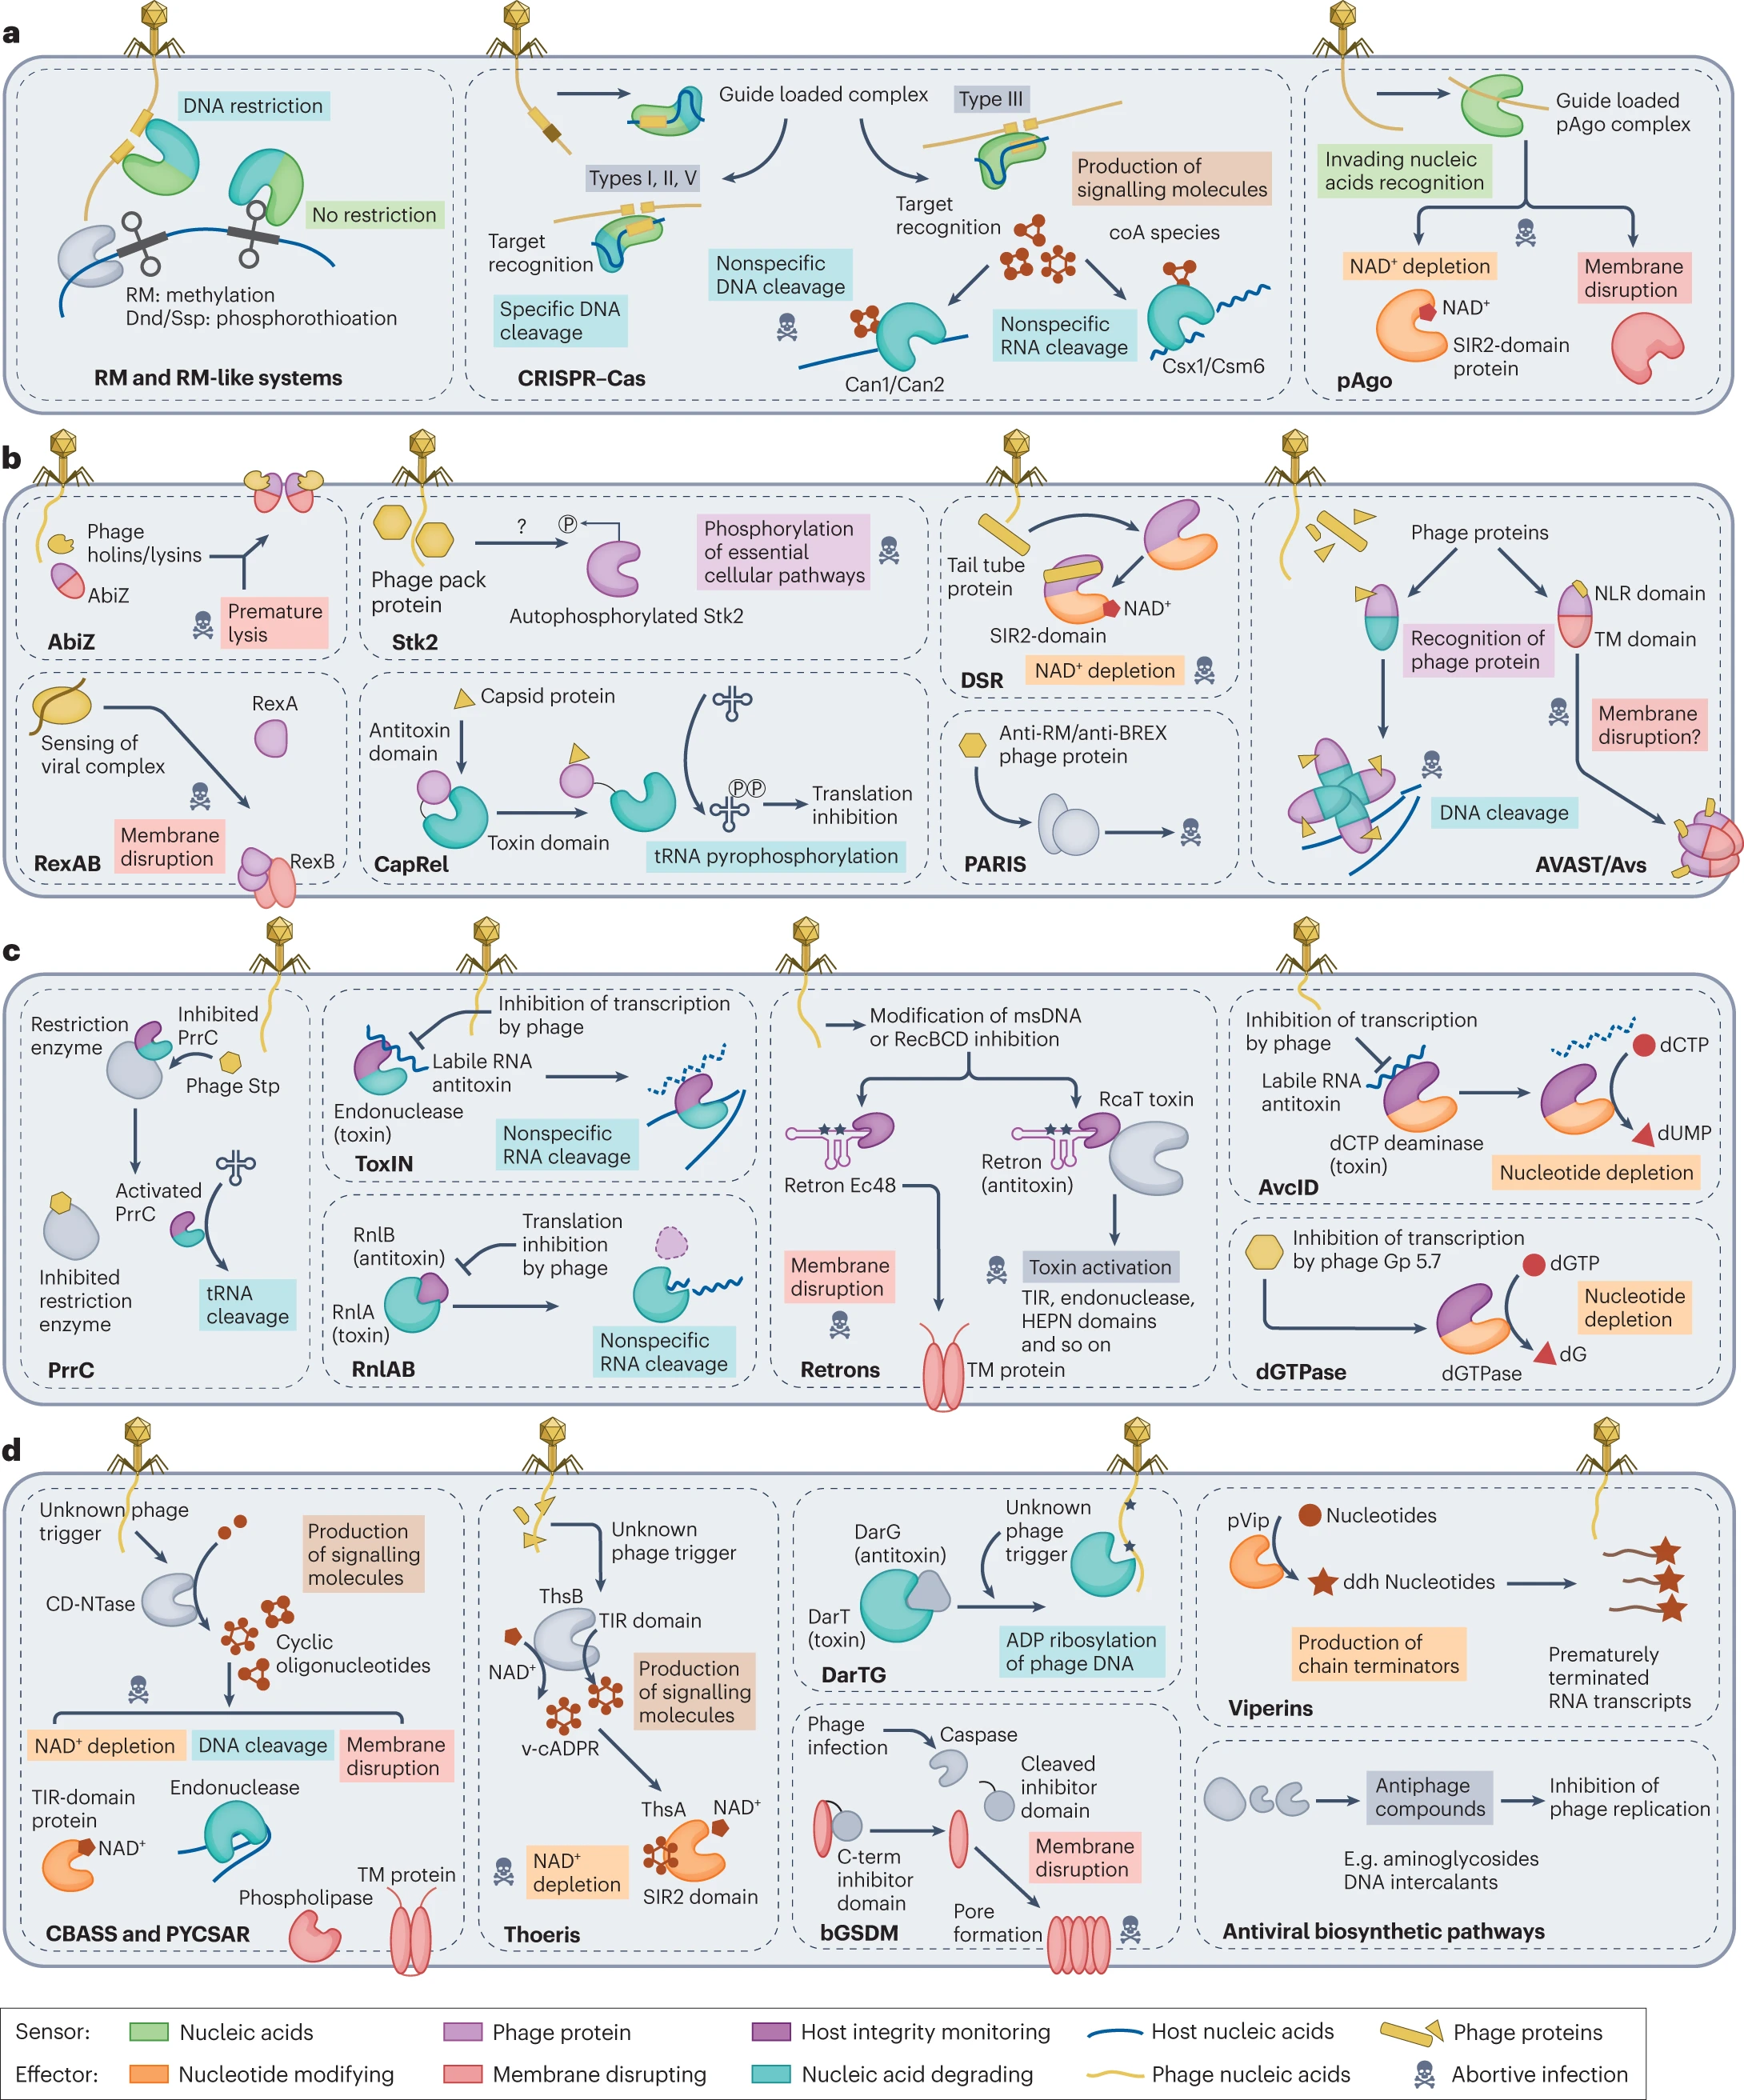
\includegraphics[width=\textwidth]{images/defensesys.png}
    \caption[Diversité des systèmes de défenses aux phages]{Diversité des systèmes de défenses aux phages. Extrait de \cite{georjon_highly_2023}}
    \label{fig:defsys}
\end{figure}

Les premiers systèmes de défense ont été identifiés dans les années 50, il s'agit des systèmes de restriction-modification (RM) \cite{bertani_host_1953}. Ces systèmes sont divisés en 2 activités (généralement 2 protéines), la reconnaissance et la scission de l'ADN étranger (REase) et la modification par méthylation (MTase) pour protéger l'ADN contre la coupure. La REase étant non spécifique, l'activité de la MTase permet de prévenir et de protéger les réplicons de l'hôte. 

C'est à partir des années 2000, que de nouveaux systèmes de défense ont été identifiés....
Un autre type de système, également connus aujourd'hui et notamment pour leur application en médecine, sont les systèmes CRISPR-Cas \cite{haft_guild_2005,barrangou_crispr_2007}. Les CRISPRs correspondent à des clusters de séquences palindromiques répétés et régulièrement espacés par des régions appelées \textit{spacer}. Certains de ces \textit{spacers} correspondent à des séquences d'ADN phagique et sera utilisé par des protéines Cas pour combattre l'infection virale. La première fonction des complexes protéiques Cas est de se lier à des transcrits de \textit{spacer} pour identifier spécifiquement l'ADN viral infectant la cellule et le découper pour l'inactiver. La seconde fonction va être de récupérer de l'ADN viral et de l'intégrer dans le chromosome entre des séquences CRISPR et en faire un \textit{spacer}. Les systèmes CRISPR-Cas permettent donc à la cellule de répondre efficacement aux infections par des phages connus, mais aussi de construire une mémoire immunitaire. 

Il existe également des systèmes d'infection abortive (Abi, pour \textit{Abortive infection} en anglais) qui entraîne la mort de l'hôte avant la réplication du phage \cite{molineux_host-parasite_1991}. Contrairement aux mécanismes précédents qui protègent l'hôte de l'infection, ces mécanismes permettent de protéger les bactéries environnantes en empêchant le phage de se multiplier. Actuellement, avec la découverte récente de nouveaux systèmes, la définition et la classification des systèmes Abi en tant que mécanisme de défense est discuté. Dans leur article, Aframian et Eldar soutiennent que l'Abi ne doit pas être considéré comme faisant partie des caractéristiques de systèmes de défense, mais comme une voie possible pour l'organisme et le phage emprunté dans certaines conditions \cite{aframian_abortive_2023}.

Aujourd'hui, plus de 150 systèmes sont référencés et pour la majorité, ils ont été découverts dans les 10 dernières années, suite à l'intérêt croissant pour les phages et leur application, mais aussi au développement de méthodes pour les détecter. En 2018, Doron, Melamed \textit{et al} \cite{doron_systematic_2018} ont identifié 26 nouveaux systèmes de défense, dont 9 qui ont pu être prouvés expérimentalement. Pour cela ils se sont basés sur un taux de colocalisation des systèmes de défense élevés dans des îlots de défense \cite{makarova_defense_2011}. À partir de là, de nombreux articles se basent sur la même stratégie pour trouver de nouveaux systèmes de défense.

Il est possible de classifier ces systèmes en 4 grandes catégories \autoref{fig:defsys} :
\begin{itemize}
    \item Les systèmes reconnaissent l'ADN des phages 
    \item Les systèmes reconnaissent les protéines de phages 
    \item Les systèmes surveillant l'intégrité de la cellule 
    \item Les autres systèmes 
\end{itemize}

Dans le même temps, avec l'émergence d'outils de détection (cf. \autoref{sec:defmet}), on s'intéresse à la distribution de ces systèmes entre et au sein des espèces procaryotes. Bernheim et Sorek \cite{bernheim_pan-immune_2020} ont montré qu'au sein d'une espèce toutes les souches ne présentent pas les mêmes systèmes et que les organismes s'échangent les systèmes par transfert horizontal. Ainsi, le système immunitaire d'un organisme correspond aux systèmes présents dans son génome et à ceux disponibles dans les autres cellules. En 2022, Tesson \textit{et al.} montre que la composition en systèmes de défense varie entre les espèces, mais aussi selon la taille du génome, le risque d'infection et le mode de vie \cite{tesson_systematic_2022}. Pour terminer, Beavogui \textit{et al.} \cite{beavogui_defensome_2024} se sont intéressé au système immunitaire dans les données de génomique environnementale et ont montré une distribution différente des systèmes de défense en fonction de l'habitat et de la géographie.

Toutes ces études ont été permises par l'arrivée de méthodes et d'outils de détection automatique des systèmes de défense dans les génomes.

\subsubsection{Méthodes et outils de détection}
\label{sec:defmet}

Les premiers outils de détection des systèmes de défenses dans les génomes se concentrait uniquement les systèmes CRISPR. Ces outils recherchait des séquences répété (CRISPR) par alignement, séparé par des séquences uniques. L'outil PILER-CR \cite{edgar_piler-cr_2007} détecte toutes les séquence répété palindromiques, puis filtre celle correspondant à des CRISPR (entre 24 et 48 pb, séparé par des séquences uniques). Puis en utilisant une méthode de graphe et de partitionnement, il identifie les CRISPR. L'outil CRT \cite{bland_crispr_2007}, utilise des k-mers pour rechercher des séquences répétées d'une taille donnée, éloigné d'une distance définie et dont la séquence est unique. Ces 2 méthodes sont rapides et ont l'intérêt de détecter toutes les séquences répétés candidate pour être des CRISPR. L'outil CRISPRFinder \cite{grissa_crisprfinder_2007}, va suivre un schéma similaire aux outils précédent, mais va introduire une notion de score, qui prend en compte le nombre de répétions, leur taille, la régularité et la taille des espacements. De plus, une fois les séquences candidates filtrées, pour améliorer sa précision, CRISPRFinder peut comparer les candidats à sa base de données de CRISPRs validées.

Avec l'accumulation des connaissances autours des CRISPRs et des séquences environnantes qui les composent, les outils vont intégrer de nouveaux critères de détection. Des outils comme CRISPRstrand\cite{alkhnbashi_crisprstrand_2014}, CRISPRDirection\cite{biswas_accurate_2014} utilise les séquences d'ARNcr\footnote{Les ARNcr, sont un type d'ARN contenant le transcrit d'une partie du CRISPR et le spacer. Ils sont utilisés dans la reconnaissance spécifique de l'ADN étranger.}, d'autres utilise les séquences leader\footnote{Une séquence séparant les CRISPR des gènes codant pour les Cas.} comme CRISPRleader \cite{alkhnbashi_characterizing_2016}. A sa sortie, MacSyFinder \cite{abby_macsyfinder_2014} intégrait une base de données HMM et de modèles CasFinder, pour identifier les protéines Cas et autres séquences connue proche pour identifier les systèmes CRISPR-Cas. En 2018, Une version hybride entre CRISPRFinder et CasFinder est proposé appelé CRISPRCasFinder \cite{couvin_crisprcasfinder_2018}. Cet outil permet de prendre en compte la structure des CRISPR et des \textit{spacers}, ainsi que les gènes environnant, pour détecter finement un contexte CRISPR-Cas.


En 2021, suite à la découverte de nombreux systèmes, l'outil PADLOC \cite{payne_identification_2021} propose l'identification de ces systèmes dans les génomes en s'appuyant sur une base de données HMM et un système de modèle, comme le propose MacSyFinder. Peu de temps après, DefenseFinder \cite{tesson_systematic_2022} est publié à son tour. PADLOC et DefenseFinder (se basant sur MacSyFinder), ont un fonctionnement similaire. Les principales différences réside dans la construction des HMMs, entièrement \textit{de novo} pour PADLOC et utilisant en partie des bases de données de protéines pour DefenseFinder; et les règles décrites dans les modèles (synténie et présence/abscence des gènes). De plus, la philosophie derrière les outils est différentes. PADLOC propose des modèles généraux, regroupement un ensemble de système proche connue, avec des règles plus flexible dans l'idée de trouver des nouveaux systèmes inconnue proche. DefenseFinder propose des modèles plus stricte, avec plus de paramètres, identifiant plus finement les systèmes. Il est donc essentiel de prendre en compte le contexte d'étude pour choisir l'outil approprié. Dans mon travail de thèse, j'ai notamment utilisé les bases de données de ces outils pour développer une méthode d'identification des systèmes dans les pangénomes. J'ai également comparé, les outils à ma méthode. À cette occasion, j'ai pu montrer que les 2 outils ne renvoie pas les mêmes résultats de prédictions. 

De la même manière que pour les autres types de systèmes, les méthodes de prédictions bénéficient des développements des modèles d'apprentissage. L'outil CRISPRidentify\cite{mitrofanov_crispridentify_2021} commence, comme ses prédécesseures, par identifier les séquences CRISPR candidate. La seconde phase, extrait différentes caractéristiques parmi les candidates (stabilité des ARNcr, similarité avec les CRISPRs connues, tailles des \textit{spacers}\dots, contenue en nucléotide AT). Enfin, un algorithme de classification, entraîné sur des données vérifiées de CRISPR, permet de valider et d'assigner un score de confiance aux candidates. Comparé aux autres outils de détection CRISPR, CRISPRidentify est plus sensible et retourne moins de faux positif. D'autres outils, comme DeepDefense \cite{hauns_deepdefense_2024} et DeepPredictor\cite{hauns_deepdefense_2024} utilise des méthodes de \textit{deeplearning}, pour la prédiction de systèmes de défense. L'intérêt de ces méthodes basé sur l'apprentissage machine est qu'elle détecte plus de systèmes et même des systèmes inconnus. Toutefois, ces méthodes sont très sensibles aux données d'apprentissage. De plus, ces méthodes demande beaucoup de ressources de calculs, et notamment, dans les exemples présentés, le nombre de génomes utilisé reste plutôt limité par rapport au nombre de génomes disponible dans les banques.